\documentclass{bmvc2k}

%% Enter your paper number here for the review copy
% \bmvcreviewcopy{??}

% \usepackage[brazilian]{babel}
\usepackage[utf8]{inputenc}
\usepackage{url}

\title{Projeto Demonstrativo 2}

% Enter the paper's authors in order
% \addauthor{Name}{email/homepage}{INSTITUTION_CODE}
\addauthor{Raphael Soares 14/0160299}{raphael.soares.1996@gmail.com}{1}

% Enter the institutions
% \addinstitution{Name\\Address}
\addinstitution{
  Departamento de Ciência da Computa\c{c}\~ao\\
  Universidade de Bras\'{\i}lia\\
  Campus Darcy Ribeiro, Asa Norte\\
  Bras\'{\i}lia-DF, CEP 70910-900, Brazil,  
}

\runninghead{Raphael, Soares Ramos}{Computer Vision Assignment -- \today}

% Any macro definitions you would like to include
% These are not defined in the style file, because they don't begin
% with \bmva, so they might conflict with the user's own macros.
% The \bmvaOneDot macro adds a full stop unless there is one in the
% text already.
\def\eg{\emph{e.g}\bmvaOneDot}
\def\Eg{\emph{E.g}\bmvaOneDot}
\def\etal{\emph{et al}\bmvaOneDot}

%-------------------------------------------------------------------------
% Document starts here
\begin{document}

\maketitle

\begin{abstract}
Este segundo projeto tem como objetivo principal a avaliação dos aspectos envolvidos em calibração de câmeras. Para isso, foi desenvolvida uma ``régua visual'' que tenta estimar a altura ou largura de um objeto através apenas da sua imagem capturada pela câmera. Ou seja, através da medida em pixels de um objeto, o programa é capaz de estimar a medida real, em centímetros, deste objeto. Para atingir esse objetivo foi necessário transformar coordenadas em pixels da imagem em coordenadas tridimensionais do mundo real usando os parâmetros extrínsecos e a matriz de parâmetros intrínsecos da câmera, que por sua vez foi obtida através da calibração da câmera realizada.
\end{abstract}

%-------------------------------------------------------------------------
\section{Introdução}
\label{sec:intro}
A visão começa com a detecção de luz do mundo. Esta luz começa com raios emanando de alguma origem, que viajam pelo espaço até atingir algum objeto. Quando esta luz atinge algum objeto, muito dela é absorvida, e o que não é absorvido nós percebemos como a cor do objeto. A luz refletida que encontra o caminho até o nosso olho (ou nossa câmera) é colecionada na nossa retina/imager (ou nosso ``filme/aparelho''). A geometria desse arranjo (particularmente da viagem dos raios do objeto através da lente em nossos olhos ou câmera e para a retina ou filme) é de grande importância para a prática de visão computacional. Um modelo simples, porém útil de como isso acontece é o modelo da câmera pinhole apresentado em~\cite{Hartley}. Infelizmente, um pinhole real não é uma boa forma de obter imagens porque ele não obtém luz suficiente para exposições rápidas e isso é um dos motivos de nossas câmeras e olhos usarem lentes, porque dessa forma podemos obter mais luz do que estaria disponível em um ponto.

Este projeto tem como objetivo usar calibração de câmeras para corrigir (matematicamente) desvios principais que o uso de lentes nos traz, as distorções. Existem dois tipos principais de distorções de lentes: radial, que é resultado da forma das lentes; e a tangencial, que surge do processo de montagem da câmera. Na teoria é possível definir lentes que não introduzem distorções, porém na prática nenhuma lente é perfeita. A calibração de câmeras é importante também, para relacionar as medidas da câmera com as medidas no mundo real tridimensional. Essa relação é importante não só porque as cenas são tridimensionais, mas porque elas também são espaços físicos com unidades físicas. Portanto, a relação entre a unidade natural da câmera (pixels) e as unidades do mundo físico (metros, por exemplo) é um componente crítico para reconstruir uma cena tridimensional ou construir uma régua visual.

%-------------------------------------------------------------------------
\section{Metodologia}
\label{sec:Methods}
Nesta seção são apresentados os métodos e procedimentos utilizados em cada um dos requisitos para obter os resultados pedidos.
\subsection{Requisito 1}
Assim como no projeto demonstrativo 1, foram usados dois booleanos \textit{x} e \textit{y} para verificar se o primeiro e o segundo clique do mouse foram dados, respectivamente. Também há um terceiro booleano \textit{z} que indica se houve ou não clique no frame em questão. O algoritmo funciona da seguinte forma:
\begin{itemize}
\item Ao dar um clique do mouse, primeiramente é verificado se \textit{x} é verdadeiro. Em caso afirmativo, \textit{y} é setado para verdadeiro e desenhamos a linha usando os pontos armazenados anteriormente.
\item Em caso negativo, setamos \textit{y} para falso.
\item Trocamos o valor verdade atual de \textit{x} caso um clique seja dado. Isso se faz necessário para o caso de haver mais de dois cliques do mouse.
\item Se houve clique então \textit{z} é setado para verdadeiro, caso contrário é setado para falso. O booleano \textit{z} é usado para desenharmos a linha nos frames seguintes mesmo que não haja clique, caso seja necessário. Para isso o passo 2 é essencial, pois precisamos saber se houveram dois cliques ou não.
\end{itemize}
O algoritmo ``apaga'' uma linha já desenhada caso um novo clique do mouse seja dado e já considera este novo clique como um primeiro clique para uma nova linha. Além disso, as coordenadas dos pixels são salvas conforme os cliques são dados. Essas coordenadas são necessárias não só para que a linha seja desenhadas nos frames seguintes do vídeo, mas também para que o cálculo da estimativa da altura ou largura do objeto seja feito no \ref{Met:Req4}.

\subsection{Requisito 2}
\label{Methods:req2}
O OpenCV~\cite{OpenCV} fornece vários algoritmos para nos ajudar a computar os parâmetros intrínsecos e o vetor de distorção. A calibração é feita via \textit{cv::calibrateCamera()}, que já fornece os vetores de translação, rotação, o vetor de distorção e a matriz com os parâmetros intrínsecos da câmera. Para cada imagem que a câmera captura de um objeto particular, nós podemos descrever a pose do objeto relativo ao sistema de coordenadas da câmera em termos da rotação e da translação. O vetor de translação é como nós representamos um deslocamento de um sistema de coordenadas para outro cuja origem é deslocada para outra localização. Ou seja, o vetor de translação é apenas o deslocamento da origem do primeiro sistema de coordenadas para o segundo. Assim, para mudar de um sistema de coordenadas centrado em um objeto para um centrado na câmera, o vetor de translação apropriado é: $\overrightarrow{T} = origin_{object} - origin_{camera}$. Dessa forma, é possível notar pela \textbf{Figura} \ref{fig:req2} que um ponto das coordenadas do objeto (ou mundo) $\overrightarrow{P_o}$ tem coordenadas $\overrightarrow{P_c}$ nas coordenadas do frame da câmera: $\overrightarrow{P_c} = R \cdot (\overrightarrow{P_o} - \overrightarrow{T})$. Esta equação combinada com as correções intrínsecas da câmera irão formar o sistema de equações que o OpenCV irá resolver. A solução para estas equações contém os parâmetros de calibração da câmera.

\begin{figure}
\begin{center}
\begin{tabular}{c}
\bmvaHangBox{\fbox{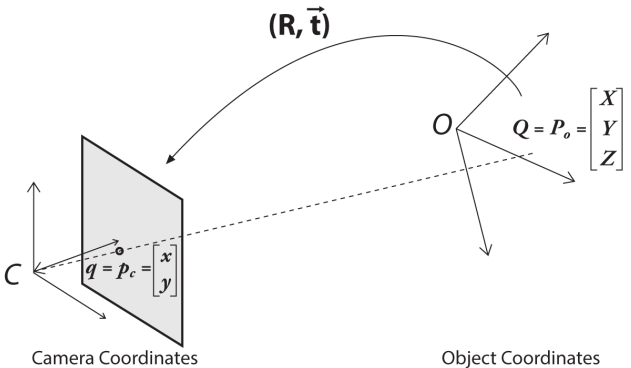
\includegraphics[width=8cm]{Figs/rot_trans.png}}} \\
\rule{0pt}{1ex}
\end{tabular}
\end{center}
\caption{Convertendo do sistema de coordenadas do objeto para o sistema de coordenadas da câmera: o ponto P no objeto é visto como o ponto p no plano da imagem; nós relacionamos o ponto p com o ponto P aplicando uma matriz de rotação R e um vetor de translação t em P.
Fonte: ~\cite{kaehler2016learning}}
\label{fig:req2}
\end{figure}

No OpenCV~\cite{opencvmanual} nós temos 4 parâmetros associados a matriz intrínseca da câmera, cinco (ou mais) parâmetros de distorção, que consistem de três (ou mais) parâmetros radiais, e dois tangenciais. Os parâmetros intrínsecos controlam a transformação linear de projeção que relacionam o objeto físico com a imagem produzida. Na teoria seria necessário apenas três pontos de cantos em um padrão conhecido para resolver os nossos 5 parâmetros de distorção. Logo, apenas uma \textit{``screenshot''} do tabuleiro de xadrez seria suficiente. Entretanto, devido ao casamento dos parâmetros intrínsecos com os extrínsecos, apenas uma \textit{``screenshot''} não é suficiente. Pode-se notar que os parâmetros extrínsecos incluem três parâmetros de translação e três de rotação dando um total de 6 por imagem do tabuleiro de xadrez. Junto com os 4 parâmetros da matriz dos intrínsecos da câmera nós temos um total de 10 que precisamos resolver, em um caso de uma única imagem, e 6 adicionais para cada imagem. Supondo que temos $N$ cantos e $K$ imagens do tabuleiro de xadrez (em posições diferentes) é necessário ter $2 \cdot N \cdot K \geq 6 \cdot K \cdot 4 ((N - 3)\cdot K \geq 2)$, onde $K \ge 1$ para resolver o problema de calibração. Entretanto, conforme apresentado em~\cite{kaehler2016learning}, para resultados de alta qualidades é necessário pelo menos 10 imagens de um xadrez 7 x 8 ou maior, na prática. Esta disparidade entre as 2 imagens na teoria, e 10 ou mais requeridas na prática, é resultado de um alto grau de sensibilidade que os parâmetros intrínsecos possuem, mesmo com pouco ruído. Por isso, nesse passo, em vez de fazer a média dos parâmetros de calibração obtidos de algumas \textit{snapshots} do tabuleiro, foram obtidas \textbf{24 snapshots/screenshots} para obter a matriz de calibração, vetores de translação, rotação e coeficientes de distorção. Sendo que os 8 primeiros \textit{snapshots} foram obtidos a uma distância de 30 cm do centro da câmera ($d_{min}$), os 8 seguintes a uma distância de 44 cm ($d_{med}$) e os 8 últimos a uma distância de 58 cm ($d_{max}$). Depois, foi calculada a média e desvio padrão para cada um dos três grupos de 8 vetores de translação obtidos com esses 24 \textit{snapshots}.

\subsection{Requisito 3}
O parâmetro \textit{objectPoints} da função \textit{cv::calibrateCamera()} foi definido da seguinte forma no programa: o primeiro canto no tabuleiro de xadrez está no ponto (0,0,0), o próximo no (0,1,0), o próximo (0,2,0), e assim em diante. Dessa forma, a escala do vetor \textit{tvec} de translação da saída da função \textit{cv::calibrateCamera} foi implicitamente alterada. Ou seja, ao definir os pontos dos cantos dos tabuleiros de xadrez desta forma, as distâncias são medidas em ``quadrados do tabuleiro''\footnote {Em contrapartida, os parâmetros da matriz intrínseca da câmera são sempre reportados em pixels}. Logo, ao calcular a norma do vetor de translação foi necessário depois multiplicar pela largura ou altura do quadrado do tabuleiro (na unidade correspondente das distâncias) para comparar com as distâncias $d_{min},\,d_{med},\,d_{max}$. 

Os parâmetros extrínsecos são os vetores de rotação e translação (\textit{tvec e rvec}), que transformam pontos definidos no \textit{frame} das coordenadas do mundo para pontos definidos no \textit{frame} da camera. Eles são saídas da função \textit{cv::calibrateCamera()} e são apresentados no terminal durante a execução do programa. Cada vetor possui 3 elementos, correspondentes aos eixos \textit{x, y, z}, e temos \textit{n} de cada um desses dois vetores, onde \textit{n} é o número de capturas do tabuleiro.

\subsection{Requisito 4}
\label{Met:Req4}
Para a imagem sem distorção, primeiro foi computado os ``\textit{undistortion maps}'' e depois foram aplicados na imagem através da função \textit{cv::remap()}. O motivo para esta separação, em vez de usar a função \textit{cv::undistort()}, é porque assim só é necessário calcular os \textit{undistortion maps} uma única vez usando os parâmetros de calibração, e depois apenas aplicá-los na imagem, conforme novos frames do vídeo vão chegando. 

Para estimar a largura/altura do objeto é necessário mapear um ponto 2D no plano da imagem para um ponto no espaço 3D. Este processo é conhecido como \textit{back-projection}, que consiste em projetar um ponto \textit{q} da imagem no conjunto de pontos do espaço 3D, sendo que os pontos 3D pertencentes a este conjunto constituem um raio no espaço, o qual passa pelo centro de projeção da câmera. Conforme apresentado por ~\cite{relatoriomoodle}, para ~\cite{phdcoord} é possível calcular o raio $Q(\lambda)$ que passa pelo centro da câmera para obter as coordenadas do mundo real usando, entre outros fatores, a matriz de rotação, a matriz com os parâmetros intrínsecos da câmera e o ponto no plano da imagem.

Contudo, como a distância $d \in \{d_{min}, d_{med}, d_{max}\} = \{30, 44, 55\}$ entre o objeto a se medir e o centro da câmera é conhecida (profundidade), e o objetivo é apenas de estimar medidas, foi usado um método mais simples de estimação das medidas do objeto~\cite{webpage}. A coordenada $X, Y, Z$ do mundo real foi obtida usando a seguinte equação: \begin{equation}
\begin{bmatrix}
X \\
Y \\
Z 
\end{bmatrix} = dK^{-1}q 
\end{equation} onde $q = (x, y, 1)^{T}$ é o ponto no plano da imagem. Aqui, a profundidade do objeto utilizada foi considerada nas distâncias $d$ pedidas. Ou seja, na teoria a parte frontal do objeto, que possui forma exata de um paralelepípedo com largura e profundidade de 2,5 cm, está a uma distância de 27,5 cm do centro da câmera para $d_{min}$, por exemplo. 

Para estimar a altura/largura de um objeto em uma imagem basta obter dois pontos no plano da imagem e calcular a distância euclidiana desses dois pontos mapeados no mundo real, independente do método utilizado. Um outro método que pode ser utilizado para estimação da pose da câmera é o apresentado por ~\cite{teofilo}, que consiste em usar a matriz de projeção para obter os parâmetros internos e externos de calibração. Além disso, usando um fator de escala é possível obter as coordenadas do mundo real correspondentes a um ponto na imagem através da matriz de projeção. Também é possível obter a posição da câmera no frame do mundo usando a transformação euclidiana inversa.

%Para câmeras baratas, nós normalmente usamos os dois primeiros termos; o primeiro deles é convencionalmente chamado de $k_1$ e o segundo $k_2$.  Para câmera mais distorcidas um terceiro termo de distorção radial é usado: $k_3$. No geral, a localização radial de um ponto no aparelho será ajustado de acordo com as seguintes equações: $$x_{corrected} = x \cdot (1 + k_1r^2 + k_2r^4 + k_3r^6)$$ e: $$y_{corrected} = y \cdot (1 + k_1r^2 + k_2r^4 + k_3r^6)$$
%
%Aqui, $(x,y)$ é a localização original (no imager) do ponto distorcido e $(x_{corrected}, y_{corrected})$ é a nova localização como resultado da correção.
%
%A distorção tangencial é caracterizada por dois parâmetros adicionais: $p_1$ e $p_2$ tal que: $$x_{\mbox{corrected}} = x + (2p_1xy + p_2(r^2 + 2x^2))$$ e: $$y_{corrected} = y + (p_1(r^2 + 2y^2) + 2p_2xy)$$
%
%Dessa forma, temos um total de 5 coeficientes de distorção requeridos. Esses 5 coeficientes de distorção são apresentados como saída do programa em uma única matriz 5 x 1 contendo $k_1,\,k_2,\,p_1,\,p_2$ e $k_3$ (nessa ordem).


%-------------------------------------------------------------------------
\section{Resultados}
\label{sec:Results}
Nesta seção são apresentados em forma de figuras e tabelas os resultados da aplicação para cada um dos requisitos. 
%-------------------------------------------------------------------------
\subsection{Requisito 1}
Apesar de não estar sendo mostrado na \textbf{Figura} \ref{fig:res:req1} o comprimento é mostrado no terminal de execução, após a linha ser desenhada. Também é mostrado os dois pixels clicados.
\begin{figure}
\begin{center}
\begin{tabular}{c}
\bmvaHangBox{\fbox{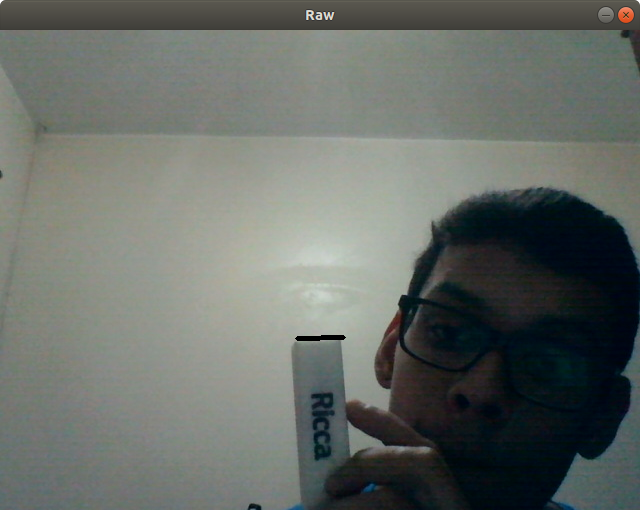
\includegraphics[width=8cm]{Figs/Req1.png}}} \\
\rule{0pt}{1ex}
\end{tabular}
\end{center}
\caption{Linha sendo desenhada na janela raw após dois cliques do mouse.}
\label{fig:res:req1}
\end{figure}

\subsection{Requisito 2}
A matriz intrínseca da câmera talvez é o resultado final mais interessante da calibração de câmeras, porque ela nos permite transformar coordenadas tridimensionais para coordenadas bidimensionais na imagem. Na \textbf{Figura} \ref{fig:res:req2} podemos ver a janela da imagem original e a sem distorção, após o processo de calibração ter sido realizado. Os resultados provenientes da calibração são apresentados no terminal do programa. Com cliques do mouse as linhas podem ser desenhadas nas duas janelas.
\begin{figure}
\begin{center}
\begin{tabular}{c}
\bmvaHangBox{\fbox{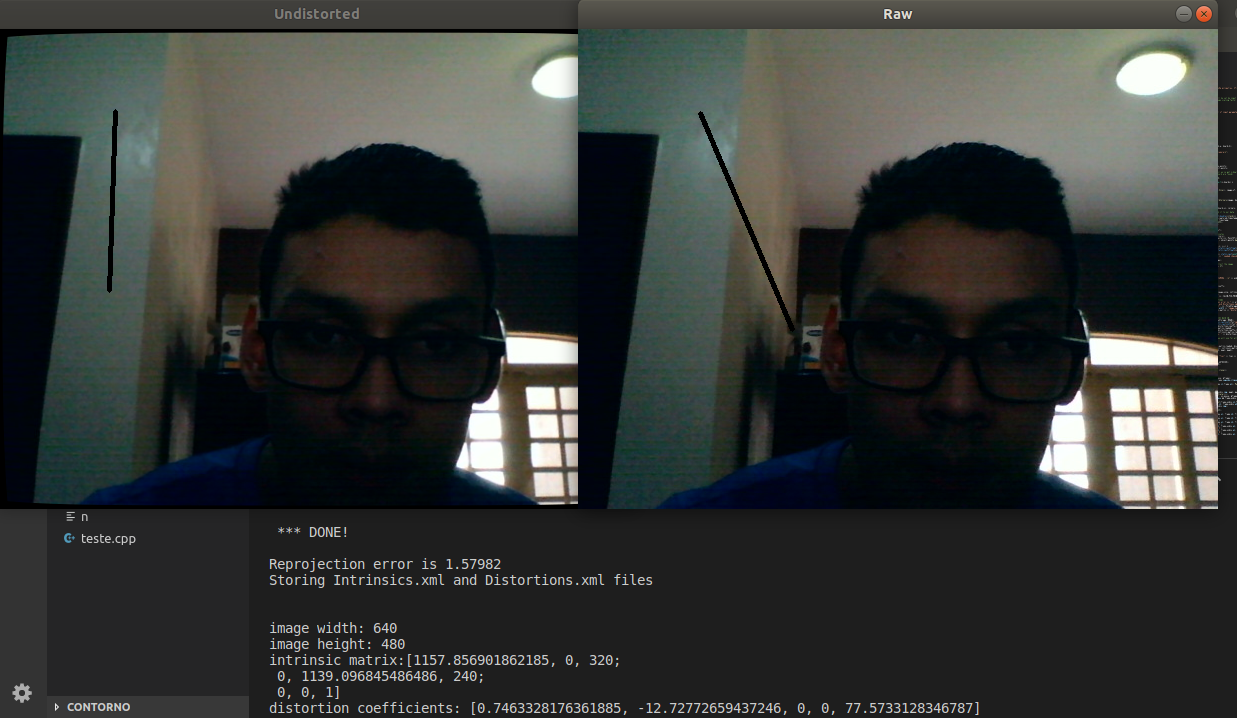
\includegraphics[width=8cm]{Figs/Req2.png}}} \\
\rule{0pt}{1ex}
\end{tabular}
\end{center}
\caption{Linhas sendo desenhadas nas janelas raw e undistorted após dois cliques do mouse em cada uma.}
\label{fig:res:req2}
\end{figure}

\subsection{Requisitos 3 e 4}
\label{res:Req4}
Os dados pedidos no requisito 3 e 4 são apresentados na \textbf{Tabela} \ref{res:Req4}. $P_1$ e $P_2$ representam as coordenadas \textit{x} e \textit{y} do primeiro e segundo pixel correspondentes ao primeiro e segundo clique do mouse dados para estimar a altura ou largura do objeto na imagem. Para $d_{min}$ a norma do vetor de translação pela calibração extrínseca é a norma dos 8 primeiros vetores de translação do total de 24, e assim em diante para as outras distâncias, conforme explicado anteriormente em \ref{Methods:req2}.

\begin{table}[h]
\label{res:table}
\caption{Tabela contendo os dados pedidos nos Requisitos 3 e 4. As medidas são fornecidas em centímetros.}
\begin{tabular}{|l|l|l|l|}
\hline
Posição                          & $d_{min} \mbox{ (cm)}$                                                                                & $d_{med} \mbox{ (cm)}$                                                                                & $d_{max}\mbox { (cm)}$                                                                                \\ \hline
$\left\|t\right\|$ da trena      & 30                                                                                       & 44                                                                                       & 58                                                                                       \\ \hline
$\left\|t\right\|$ da calibração & \begin{tabular}[c]{@{}l@{}}Média = 35.84394\\ $\sigma = 19.73154$\end{tabular}           & \begin{tabular}[c]{@{}l@{}}Média = 46.44475\\ $\sigma = 24.78756$\end{tabular}           & \begin{tabular}[c]{@{}l@{}}Média = 60.49741\\ $\sigma = 32.18481$\end{tabular}           \\ \hline
$I_{raw,centre}$                 & \begin{tabular}[c]{@{}l@{}}2.330139\\ $P_1$ = (296,249)\\ $P_2$ = (359,254)\end{tabular} & \begin{tabular}[c]{@{}l@{}}2.487273\\ $P_1$ = (264,245)\\ $P_2$ = (310,245)\end{tabular} & \begin{tabular}[c]{@{}l@{}}2.356549\\ $P_1$ = (315,286)\\ $P_2$ = (348,288)\end{tabular} \\ \hline
$I_{raw,perifery}$               & \begin{tabular}[c]{@{}l@{}}2.543802\\ $P_1$ = (17,292)\\ $P_2$ = (86,292)\end{tabular}   & \begin{tabular}[c]{@{}l@{}}2.604700\\ $P_1$ = (50,298)\\ $P_2$ = (98,302)\end{tabular}   & \begin{tabular}[c]{@{}l@{}}2.712342\\ $P_1$ = (280,373)\\ $P_2$ = (330,373)\end{tabular} \\ \hline
$I_{undistorted, centre}$        & \begin{tabular}[c]{@{}l@{}}2.433202\\ $P_1$ = (242,222)\\ $P_2$ = (308,222)\end{tabular} & \begin{tabular}[c]{@{}l@{}}2.379765\\ $P_1$ = (277,254)\\ $P_2$ = (321,255)\end{tabular} & \begin{tabular}[c]{@{}l@{}}2.494646\\ $P_1$ = (288,299)\\ $P_2$ = (323,299)\end{tabular} \\ \hline
$I_{undistorted, perifery}$      & \begin{tabular}[c]{@{}l@{}}2.618607\\ $P_1$ = (20,278)\\ $P_2$ = (91,280)\end{tabular}   & \begin{tabular}[c]{@{}l@{}}2.541938\\ $P_1$ = (133,286)\\ $P_2$ = (180,287)\end{tabular} & \begin{tabular}[c]{@{}l@{}}2.498846\\ $P_1$ = (173,278)\\ $P_2$ = (208,280)\end{tabular} \\ \hline
\end{tabular}
\end{table}

%-------------------------------------------------------------------------
\section{Discussões e Conclusões}
\label{sec:Conclusion}
%-------------------------------------------------------------------------
Para distorções radiais, a distorção é 0 no centro óptico do aparelho e cresce assim que movemos para a periferia. Na prática, esta distorção é pequena e pode ser caracterizada por poucos termos de uma expansão da série de Taylor em torno de $r = 0$. Isso explica porque as medidas do objeto tiradas próximo ao centro da imagem se aproximam mais da medida real $l, \mbox{ onde } l = 2.5 \mbox{ cm }$. Além disso, algumas medidas da largura poderiam ser mais precisas se uma linha exatamente reta pudesse ser desenhada. Por exemplo, em $I_{raw,centre}$ para $d_{min}$ a coordenada \textit{y}, que corresponde a altura, não deveria ser alterada. Entretanto, podemos observar que as medidas estimadas foram bastante próximas da medida (largura l) real. Os resultados foram satisfatórios. 

\bibliography{refs}
\end{document}